\documentclass[letterpaper,openany,oneside,twocolumn]{book}

\newcommand{\PATH}{../../}

\usepackage{\PATH templates/utilities/m4rz-fonts}
\usepackage{\PATH templates/utilities/m4rz-colors}

\usepackage[justified]{\PATH templates/template_dnd/dnd}

\usepackage{\PATH templates/template_character-sheet/character-sheet-stylesheet}
\usepackage{\PATH templates/template_magic-item/magic-items_commands}

\setlength\oddsidemargin{\dimexpr(\paperwidth-\textwidth)/2 - 1in\relax}
\setlength\evensidemargin{\oddsidemargin}

% Headline
\CharacterName{Sylvana Stormshot}

\Class{Fighter}
\Level{3}
\Background{Wildspacer}
\PlayerName{M4RZ}
\Race{Owlin}
\Alignment{Lawful Evil}
\XP{}

% Ability scores (correct scores, no modifiers are automatically applied)
% Modifiers, Saving Throws and Skills are calculated automatically
\StrengthRolledScore{12}
\DexterityRolledScore{15}
\ConstitutionRolledScore{12}
\IntelligenceRolledScore{13}
\WisdomRolledScore{12}
\CharismaRolledScore{10}

\StrengthScoreBonus{0}
\DexterityScoreBonus{2} % Owlin-Race +2
\ConstitutionScoreBonus{0}
\IntelligenceScoreBonus{1} % Owlin-Race +1
\WisdomScoreBonus{0}
\CharismaScoreBonus{0}

\calculateAbilityScores{}

\StrengthScore{12}
\DexterityScore{17}
\ConstitutionScore{14}
\IntelligenceScore{14}
\WisdomScore{12}
\CharismaScore{10}

% Proficiencies (Proficient = 'P', Expertise = 'E', otherwise = '')
\StrengthProficiency{P}
\DexterityProficiency{}
\ConstitutionProficiency{P}
\IntelligenceProficiency{}
\WisdomProficiency{}
\CharismaProficiency{}

\AcrobaticsProficiency{P}
\AnimalHandlingProficiency{}
\ArcanaProficiency{P}
\AthleticsProficiency{P}
\DeceptionProficiency{}
\HistoryProficiency{}
\InsightProficiency{}
\IntimidationProficiency{}
\InvestigationProficiency{}
\MedicineProficiency{}
\NatureProficiency{}
\PerceptionProficiency{P}
\PerformanceProficiency{}
\PersuasionProficiency{}
\ReligionProficiency{}
\SleightOfHandProficiency{}
\StealthProficiency{P}
\SurvivalProficiency{P}

% ABILITY MODIFIERS BONUS
\StrengthModifierBonus{0}
\DexterityModifierBonus{0}
\ConstitutionModifierBonus{0}
\IntelligenceModifierBonus{0}
\WisdomModifierBonus{0}
\CharismaModifierBonus{0}

\Inspiration{}
\Proficiency{+2}
\PassivePerceptionModifier{0}

% Armor Class is not automatically calculated
\ArmorClass{14}
\InitiativeModifier{0}
\Speed{30}
\MaxHitPointsRolled{27} % Without Constitution Bonus, is added automatically
\CurrentHitPoints{}
\TemporaryHitPoints{}
\HitDice{d10}
\HitDiceSpent{0}

\CP{}
\SP{}
\EP{}
\GP{140}
\PP{}

% Weapon Arsenal
\addWeaponStatistic{Longbow}{SylvanaStormshot}{DEX}{P}{2}{1d8 p}
\addWeaponStatistic{Rapier}{SylvanaStormshot}{DEX}{P}{0}{1d8 s}
\addWeaponStatistic{Handaxe}{SylvanaStormshot}{STR}{P}{0}{1d6 s}
\addWeaponStatistic{Unarmed Strike}{SylvanaStormshot}{STR}{P}{0}{\intcalcAdd{1}{\calculateModifier{\StrengthScoreValue}} b}

\AttacksAdditional{
	\textbf{Longbow} (150/600), 20 Arrows\\
	\textbf{Arcane Shot}
	\begin{itemize}
		\item Banishing Arrow
		\item Shadow Arrow
	\end{itemize}
	\textbf{Rapier}\\
	\textbf{2 Handaxes} (20/60)
}

\OtherProficienciesLanguages{
\textbf{Languages:}\\Common, Sylvan\\
\textbf{Armor:}\\All armor, Shields\\
\textbf{Weapons:}\\Simple Weapons, Martial Weapons\\
\textbf{Tools:}\\Navigator's Tools
}

\Equipment{
	Shield, Leather Armor
}
\Clutter{
	backpack, crowbar, hammer, 10 pitons, 10 torches, 10 days of rations, a waterskin, 2x 50 feet of hempen rope, belaying pin (club), set of traveler's clothes, grappling hook
}

\PersonalityTraits{
	Sylvana tends to be a quiet and introspective individual. She often takes moments to observe the world around her, appreciating the beauty of nature and reflecting on her experiences.
}

\Ideals{
	Sylvana believes in protecting the delicate balance of the forest, its creatures, and the magic that sustains it.
}

\Bonds{
	Sylvana carries the memory of her mentor, Thalindra, in her heart. Thalindra's guidance and sacrifice continue to inspire and drive her.
}

\Flaws{
	Sylvana's pursuit of vengeance against Xerathax can sometimes blind her to other priorities or lead her into reckless situations.
}

\FeaturesTraits{
\textbf{Owlin Traits}
\begin{itemize}
	\item Darkvision
	\item Flight
	\item Silent Feathers
\end{itemize}
\textbf{Sharpshooter}\\
\textbf{Wildspacer}
\begin{itemize}
	\item Close Encounter
	\item Wildspace Adaptation
\end{itemize}
\textbf{Fighter Traits}
\begin{itemize}
	\item Fighting Style
	\item Second Wind
	\item Action Surge
	\item Arcane Archer
	\begin{itemize}
		\item Arcane Archer Lore
		\item Arcane Shot
	\end{itemize}
\end{itemize}
}

% Appearance

\Age{54}
\Height{5'8''}
\Weight{120lbs}
\Eyes{Gray}
\Skin{Beige-Feathered Owlin}
\Hair{}

% background

\CharacterAppearance{}{
	\hspace*{-1.65em}\begin{tabular}{p{100pt}p{70pt}}
		\begin{tabular}{p{80pt}}\vspace*{-1.25em}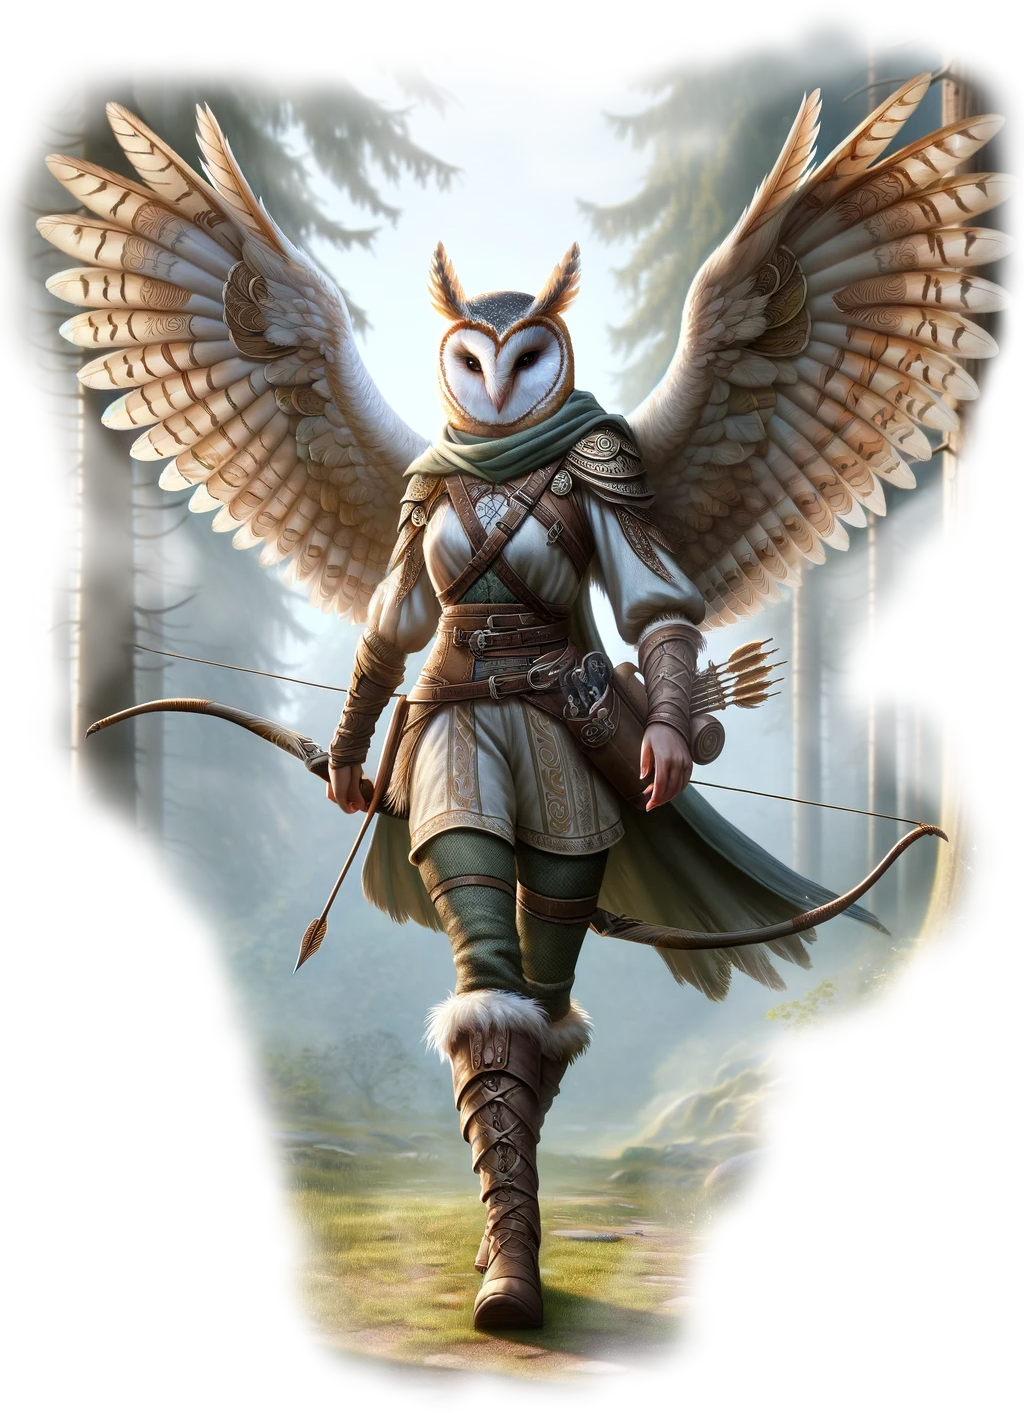
\includegraphics[width=120pt, height=140pt, keepaspectratio]{images/Sylvana_Stormshot(2).png}\end{tabular}
		&
		\hspace*{-1.6em}\begin{tabular}{>{\raggedleft}p{72pt}}Sylvana Stormshot is a graceful Owlin with beige feathers that provide excellent forest camouflage. Her forest-green eyes reflect keen perception, and\linebreak \end{tabular}
	\end{tabular}\\\vspace*{-1.6em}\hfill\\
	she's often seen in a flowing blue kimono adorned with nature-inspired patterns. She carries an air of quiet confidence, embodying the harmony of natural beauty and arcane power.
}{}{}{}
\AdditionalFeaturesAndTraits{
	Sylvana's presence seems to harmonize with the natural world around her. When she walks through the forest, the birds sing more melodiously, and the leaves rustle in harmony. Her affinity with nature often leaves those she encounters with a sense of tranquility and wonder.\\
	Sylvana's feathers are imbued with a natural resilience. They shimmer with an iridescent sheen, and they help protect her from harsh weather conditions, keeping her warm in the cold and cool in the heat. Her feathers also shed water effortlessly, allowing her to stay dry even in heavy rain.\\
	Sylvana's deep connection to the forest grants her unique insights into its secrets. She can discern the age of trees, identify rare herbs, and navigate through the thickest undergrowth with ease. Her understanding of the forest's history and the creatures that dwell within it is unparalleled.\\
	Sylvana's eyes have a keen and piercing quality. They can spot the subtlest movements in the foliage and discern even the faintest sounds. Her gaze is intense yet captivating, revealing her thoughtful and observant nature.
}
\Characterbackground{
	Sylvana Stormshot was born into a peaceful Owlin community nestled deep within an ancient forest. From a young age, her affinity for archery was evident, and she honed her skills as a hunter and protector of her woodland home.
	
	\paragraph*{Traumatic Event} Sylvana's life took a dark turn when a malevolent Beholder, known as Xerathax the Eye Tyrant, descended upon the forest. Xerathax's presence corrupted the once-vibrant flora and fauna, transforming them into grotesque aberrations. The Beholder's relentless pursuit of magical knowledge and power threatened not only Sylvana's home but the entire region.

	During a harrowing confrontation with Xerathax, Sylvana's village came under attack. The Beholder's anti-magic eye nullified the abilities of the Owlin's fellow warriors, leaving them defenseless. Sylvana's beloved mentor, an elder Owlin archer named Thalindra, sacrificed herself to protect her from Xerathax's devastating eye rays. Her sacrifice allowed Sylvana to escape the encounter, but she was left traumatized by the loss of her mentor and the devastation of her home.
}
\Treasure{
	\textbf{1. Thalindra's Feathered Quill:} This delicate quill, crafted from one of Thalindra's own feathers, serves as both a symbol of Sylvana's mentor and a tool for writing and sketching in her journal. It holds sentimental value, carrying memories of their time together and the knowledge Thalindra imparted.\\\\
	\textbf{2. Handwoven Dreamcatcher:} A meticulously handwoven dreamcatcher made from natural materials found in her forest. Sylvana believes that it helps protect her dreams from dark influences and connects her with the dream realm, where she often gains insights and guidance from the spirits of the forest.\\\\
	\textbf{3. Bound Herbal Grimoire:} A meticulously hand-bound grimoire containing a wealth of knowledge about rare herbs, magical plants, and their properties. It serves as both a guide to her herbalism and a repository of the forest's secrets.
}
\AlliesAndOrganizations{
	The Sylvan Wardens are a secretive and ancient order of guardians sworn to protect the sanctity of the natural world. Nestled deep within the heart of the ancient forest that Sylvana calls home, this organization has existed for generations. Its members, drawn from various woodland races including Owlin, Elves, and Fey creatures, share a deep bond with nature and are entrusted with the sacred task of safeguarding the forest and its inhabitants.\\
	\textbf{Alliances and Diplomacy:}\\
	The Sylvan Wardens maintain peaceful relationships with the fey creatures of the forest, local elven communities,\linebreak
}{
	and druidic circles. They occasionally form alliances with neighboring human settlements that respect nature's balance.
}
\OrganizationName{Sylvan Warden}
\OrganizationSymbol{images/Sylvan_Warden.png}

% Magic

%\SpellcastingClass{}
%\SpellcastingAbility{} % STR, DEX, CON, INT, WIS, CHA
%\SpellSaveDCModifier{0} % any modifier that isn't contained in "8 + Ability Modifier + Proficiency Bonus"
%\SpellAttackModifier{0} % any modifier that isn't contained in "Ability Modifier + Proficiency Bonus"
%
%\CantripSlotA{Cantrip A}
%
%\FirstLevelSpellSlotsTotal{1}
%\FirstLevelSpellSlotA{Spell 1.A}
%\FirstLevelSpellSlotB{Spell 1.B}
%
%\SecondLevelSpellSlotsTotal{2}
%\SecondLevelSpellSlotA{Spell 2.A}
%\SecondLevelSpellSlotB{Spell 2.B}

\begin{document}

\newgeometry{left=0cm,right=0cm,top=0cm,bottom=0cm}
\onecolumn


% CHARACTER PAGE
\rendercharactersheet

% BACKSTORY PAGE
\renderbackgroundsheet

% SPELLCASTING PAGE
%\renderspellsheet


\restoregeometry
\twocolumn

\chapter*{Features, Magic Items and Spells}

\section*{Owlin Traits}
Distant kin of giant owls from the Feywild, owlin come in many shapes and sizes, from petite and fluffy to wide-winged and majestic. Owlin have arms and legs like other Humanoids, as well as wings that extend from their back and shoulders.

Like owls, owlin are graced with feathers that make no sound when they move or fly, making it easy for them to sneak up on you in the library.

Your owlin character might be nocturnal. Or perhaps your character is simply prone to rise later, embodying the common nickname of night owl.
\subsection*{Darkvision}
You can see in dim light within 120 feet of yourself as if it were bright light and in darkness as if it were dim light. You discern colors in that darkness only as shades of gray.
\subsection*{Flight}
Thanks to your wings, you have a flying speed equal to your walking speed. You can't use this flying speed if you're wearing medium or heavy armor.
\subsection*{Silent Feathers}
You have proficiency in the Stealth skill.

\section*{Sharpshooter}
You have mastered ranged weapons and can make shots that others find impossible. You gain the following benefits:
\begin{itemize}
	\item Attacking at long range doesn't impose disadvantage on your ranged weapon attack rolls.
	\item Your ranged weapon attacks ignore half and three-quarters cover.
	\item Before you make an attack with a ranged weapon that you are proficient with, you can choose to take a -5 penalty to the attack roll. If that attack hits, you add +10 to the attack's damage.
\end{itemize}

\section*{Wildspacer}
You were raised in the void of Wildspace - home to asteroid miners, moon farmers, and other hardy folk. Perhaps you grew up in a far-flung settlement such as the Rock of Bral, or you spent your early years on the crew of a spelljamming ship, performing helpful chores such as swabbing the deck, loading and offloading cargo, and scraping barnacles off the hull.

Whatever your history, life in Wildspace has toughened you so well that you are as brave as a miniature giant space hamster when it comes to facing the terrors and other challenges of the airless night.
\subsection*{Close Encounter}
You had a harrowing encounter with one of Wildspace's many terrors. You escaped with your life, but the encounter left you with a scar or two, or perhaps a recurring nightmare. Roll on the Close Encounter table to determine which creature nearly got the best of you.
\begin{DndTable}[header=Close Encounter]{lXX}
			& \textbf{d10}  	&\textbf{Creature}	\\
$\bullet$	& 1					&Beholder			\\
			& 2					&Cosmic Horror		\\
			& 3					&Feyr				\\
			& 4					&Lunar Dragon		\\
			& 5					&Mind Flayer		\\
			& 6					&Neh-thalggu		\\
			& 7					&Neogi				\\
			& 8					&Space Clown		\\
			& 9					&Vampirate			\\
			& 10				&Void Scavver		\\
\end{DndTable}
\subsection*{Wildspace Adaptation}
You gain the Tough feat. In addition, you learned how to adapt to zero gravity. Being weightless doesn’t give you disadvantage on any of your melee attack rolls.
\paragraph*{Tough}
Your hit point maximum increases by an amount equal to twice your level when you gain this feat. Whenever you gain a level thereafter, your hit point maximum increases by an additional 2 hit points.

\section*{Fighter Traits}
Fighters share an unparalleled mastery with weapons and armor, and a thorough knowledge of the skills of combat. They are well acquainted with death, both meting it out and staring it defiantly in the face.
\subsection*{Fighting Style}
You adopt a particular style of fighting as your specialty. Choose one of the following options. You can't take a Fighting Style option more than once, even if you later get to choose again.
\paragraph*{Archery}
You gain a +2 bonus to attack rolls you make with ranged weapons.
\subsection*{Second Wind}
You have a limited well of stamina that you can draw on to protect yourself from harm. On your turn, you can use a bonus action to regain hit points equal to 1d10 + your fighter level.

Once you use this feature, you must finish a short or long rest before you can use it again.
\subsection*{Action Surge}
Starting at 2nd level, you can push yourself beyond your normal limits for a moment. On your turn, you can take one additional action.

Once you use this feature, you must finish a short or long rest before you can use it again. Starting at 17th level, you can use it twice before a rest, but only once on the same turn.
\subsection*{Arcane Archer}
\paragraph*{Arcane Archer Lore}
At 3rd level, you learn magical theory or some of the secrets of nature – typical for practitioners of of this elven martial tradition. You choose to gain proficiency in either the Arcana or the Nature skill, and you choose to learn either the Prestidigitation or Druidcraft cantrip.
\paragraph*{Arcane Shot}
At 3rd level, you learn to unleash special magical effects with some of your shots. When you gain this feature, you learn two Arcane Shot options of your choice (see "Arcane Shot Options" below).

Once per turn when you fire an arrow from a shortbow or longbow as part of the Attack action, you can apply one of your Arcane Shot options to that arrow. You decide to use the option when the arrow hits, unless the option doesn’t involve an attack roll. You have two uses of this ability, and you regain all expended uses of it when you finish a short or long rest.

You gain an additional Arcane Shot option of your choice when you reach certain levels in this class: 7th, 10th, 15th, and 18th level. Each option also improves when you become an 18th-level fighter.
\subsection*{Arcane Shot Options}
The Arcane Shot feature lets you choose options for it at certain levels. The options are presented here in alphabetical order. They are all magical effects, and each one is associated with one of the schools of magic.

If an option requires a saving throw, your Arcane Shot save DC equals 8 + your proficiency bonus + your Intelligence modifier.\\\\
\textbf{Save DC: \intcalcAdd{8}{\intcalcAdd{\ProficiencyValue}{\calculateModifier{\IntelligenceScoreValue}}}}

\eject

\paragraph{Banishing Arrow} You use abjuration magic to try to temporarily banish your target to a harmless location in the Feywild. The creature hit by the arrow must also succeed on a Charisma saving throw or be banished. While banished in this way, its speed is 0, and it is incapacitated. At the end of its next turn, the target reappears in the space it vacated or in the nearest unoccupied space if that space is occupied.

After you reach 18th level in this class, a target also takes 2d6 force damage when the arrow hits it.

\paragraph{Beguiling Arrow} Your enchantment magic causes this arrow to temporarily beguile its target. The creature hit by the arrow takes an extra 2d6 psychic damage, and choose one of your allies within 30 feet of the target. The target must succeed on a Wisdom saving throw, or it is charmed by the chosen ally until the start of your next turn. This effect ends early if the chosen ally attacks the charmed target, deals damage to it, or forces it to make a saving throw.

The psychic damage increases to 4d6 when you reach 18th level in this class.

\paragraph{Bursting Arrow} You imbue your arrow with force energy drawn from the school of evocation. The arrow detonates after your attack. Immediately after the arrow hits the creature, the target and all other creatures within 10 feet of it take 2d6 force damage each.

The force damage increases to 4d6 when you reach 18th level in this class.

\paragraph{Enfeebling Arrow} You weave necromantic magic into your arrow. The creature hit by the arrow takes an extra 2d6 necrotic damage. The target must also succeed on a Constitution saving throw, or the damage dealt by its weapon attacks is halved until the start of your next turn.

The necrotic damage increases to 4d6 when you reach 18th level in this class.

\paragraph{Grasping Arrow} When this arrow strikes its target, conjuration magic creates grasping, poisonous brambles, which wrap around the target. The creature hit by the arrow takes an extra 2d6 poison damage, its speed is reduced by 10 feet, and it takes 2d6 slashing damage the first time on each turn it moves 1 foot or more without teleporting. The target or any creature that can reach it can use its action to remove the brambles with a successful Strength (Athletics) check against your Arcane Shot save DC. Otherwise, the brambles last for 1 minute or until you use this option again.

The poison damage and slashing damage both increase to 4d6 when you reach 18th level in this class.

\eject

\paragraph{Piercing Arrow} You use transmutation magic to give your arrow an ethereal quality. When you use this option, you don’t make an attack roll for the attack. Instead, the arrow fires forward in a line, which is 1 foot wide and 30 feet long, before disappearing. The arrow passes harmlessly through objects, ignoring cover. Each creature in that line must make a Dexterity saving throw. On a failed save, a creature takes damage as if it were hit by the arrow, plus an extra 1d6 piercing damage. On a successful save, a target takes half as much damage.

The piercing damage increases to 2d6 when you reach 18th level in this class.

\paragraph{Seeking Arrow} Using divination magic, you grant your arrow the ability to seek out your target, allowing the arrow to curve and twist its path in search of its prey. When you use this option, you don’t make an attack roll for the attack. Instead, choose one creature you have seen in the past minute. The arrow flies toward that creature, moving around corners if necessary and ignoring three-quarters cover and half cover. If the target is within the weapon’s range and there is a path large enough for the arrow to travel to the target, the target must make a Dexterity saving throw. On a failed save, it takes damage as if it were hit by the arrow, plus an extra 1d6 force damage, and you learn the target’s current location. On a successful save, the target takes half as much damage, and you don’t learn its location.

The force damage increases to 2d6 when you reach 18th level in this class.

\paragraph{Shadow Arrow} You weave illusion magic into your arrow, causing it to occlude your foe’s vision with shadows. The creature hit by the arrow takes an extra 2d6 psychic damage, and it must succeed on a Wisdom saving throw or be unable to see anything farther than 5 feet away until the start of your next turn.

The psychic damage increases to 4d6 when you reach 18th level in this class.

\vfill\eject

\section*{Miscellaneous}
\subsection*{Attack and Damage Rolls}
\subsubsection*{Melee Weapons}
\paragraph*{Attack Roll}\hfill\\
\underline{\textit{Rapier (Finesse):}}\\
1d20 + DEX-Modifier + Proficiency Modifier\\
\indent Current Max: \intcalcAdd{20}{\intcalcAdd{\calculateModifier{\DexterityScoreValue}}{\ProficiencyValue}}
\\
\underline{\textit{Handaxe (Throwable):}}\\
1d20 + STR-Modifier + Proficiency Modifier\\
\indent Current Max (melee): \intcalcAdd{20}{\intcalcAdd{\calculateModifier{\StrengthScoreValue}}{\ProficiencyValue}}\\
\indent Current Max (thrown): \intcalcAdd{20}{\intcalcAdd{\calculateModifier{\StrengthScoreValue}}{\ProficiencyValue}}
\paragraph*{Damage Roll}\hfill\\
\underline{\textit{Rapier (Finesse):}}\\
1d8 + DEX-Modifier\\
\indent Current Max: \intcalcAdd{8}{\calculateModifier{\DexterityScoreValue}}
\\
\underline{\textit{Handaxe (Throwable):}}\\
1d6 + STR-Modifier\\
\indent Current Max (melee): \intcalcAdd{6}{\calculateModifier{\StrengthScoreValue}}\\
\indent Current Max (thrown): \intcalcAdd{6}{\calculateModifier{\StrengthScoreValue}}
\subsubsection*{Ranged Weapons}
\paragraph*{Attack Roll}\hfill\\
\underline{\textit{Longbow:}}\\
1d20 + DEX-Modifier + Proficiency Modifier\\
\indent Current Max: \intcalcAdd{20}{\intcalcAdd{\calculateModifier{\DexterityScoreValue}}{\ProficiencyValue}}
\paragraph*{Damage Roll}\hfill\\
\underline{\textit{Longbow:}}\\
1d8 + DEX-Modifier\\
\indent Current Max: \intcalcAdd{8}{\calculateModifier{\DexterityScoreValue}}
\subsubsection*{Special Attacks}
\paragraph*{Attack Roll}\hfill\\
\underline{\textit{Unarmed Strike:}}\\
1d20 + STR-Modifier + Proficiency Modifier\\
\indent Current Max: \intcalcAdd{20}{\intcalcAdd{\calculateModifier{\StrengthScoreValue}}{\ProficiencyValue}}
\paragraph*{Damage Roll}\hfill\\
\underline{\textit{Unarmed Strike:}}\\
1 + STR-Modifier\\
\indent Current Max: \intcalcAdd{1}{\calculateModifier{\StrengthScoreValue}}

\end{document}
